\chapter{Umsetzung}
    Die Entwicklung der Platzierungssoftware erfolgte in Java-SE 11.
    Der grobe Ablauf des Programmes besteht darin, die Netzliste sowie die fixierten Pads
    einzulesen und daraus einen Graphen zu erstellen.
    Dadurch, dass es im Praktikum nur eine relevante FPGA-Architektur zu betrachten gab,
    wurde vom Einlesen der *.arch Datei abgesehen und die benötigten Parameter wurden über
    Konstanten direkt im Programmcode abgelegt. Wurde der Graph erfolgreich erstellt wird
    eine Initialplatzierung vorgenommen. 
    Kapitel (\ref{sec:init}) beschreibt die vom Grundalgorithmus abweichende Vorgehensweise
    um die Ergebnisse der Platzierung zu optimieren. Nach Abschluss der Initialplatzierung
    beginnt die eigentliche Optimierung der Platzierung. Kapitel (\ref{sec:algo}) geht dabei auf die genauen
    Einzelheiten des Algorithmus ein.
    Nach Abschluss des Algorithmus wird aus der aktuellen Platzierung die
    Platzierungsdatei erstellt und ausgegeben.


    \begin{figure}[H]
        \centering
        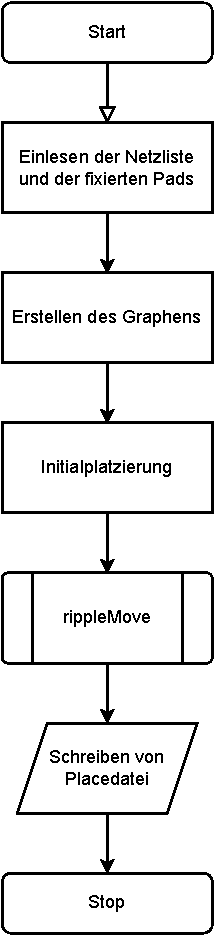
\includegraphics[scale=0.75]{img/Programm-flowchart.pdf}
        \caption{Programmablaufplan}
        \label{fig:program-flowchart}
    \end{figure}

        

    \section{Programmstruktur}

        Abbildung (\ref{fig:uml}) zeigt das UML-Diagramm des Programmes.
        Die Hauptlogik des Programmes befindet sich in der FPGA-Klasse,
        die zuständig für die Platzierung der Logikblöcke ist.
        Als wichtigste Komponente gilt der Graph, der durch die eingelesenen Blöcke sowie die
        fixierten Pads erstellt wird und der FPGA-Instanz beim Instanziieren übergeben wird.
        Über die Methoden \textit{initPlace} oder \textit{randomPlace} wird eine Initialplatzierung vorgenommen.
        Des Weiteren wird über die Methode \textit{rippleMove} die eigentliche Optimierung der Platzierung
        vorgenommen.
        \begin{figure}[H]
            \centering
            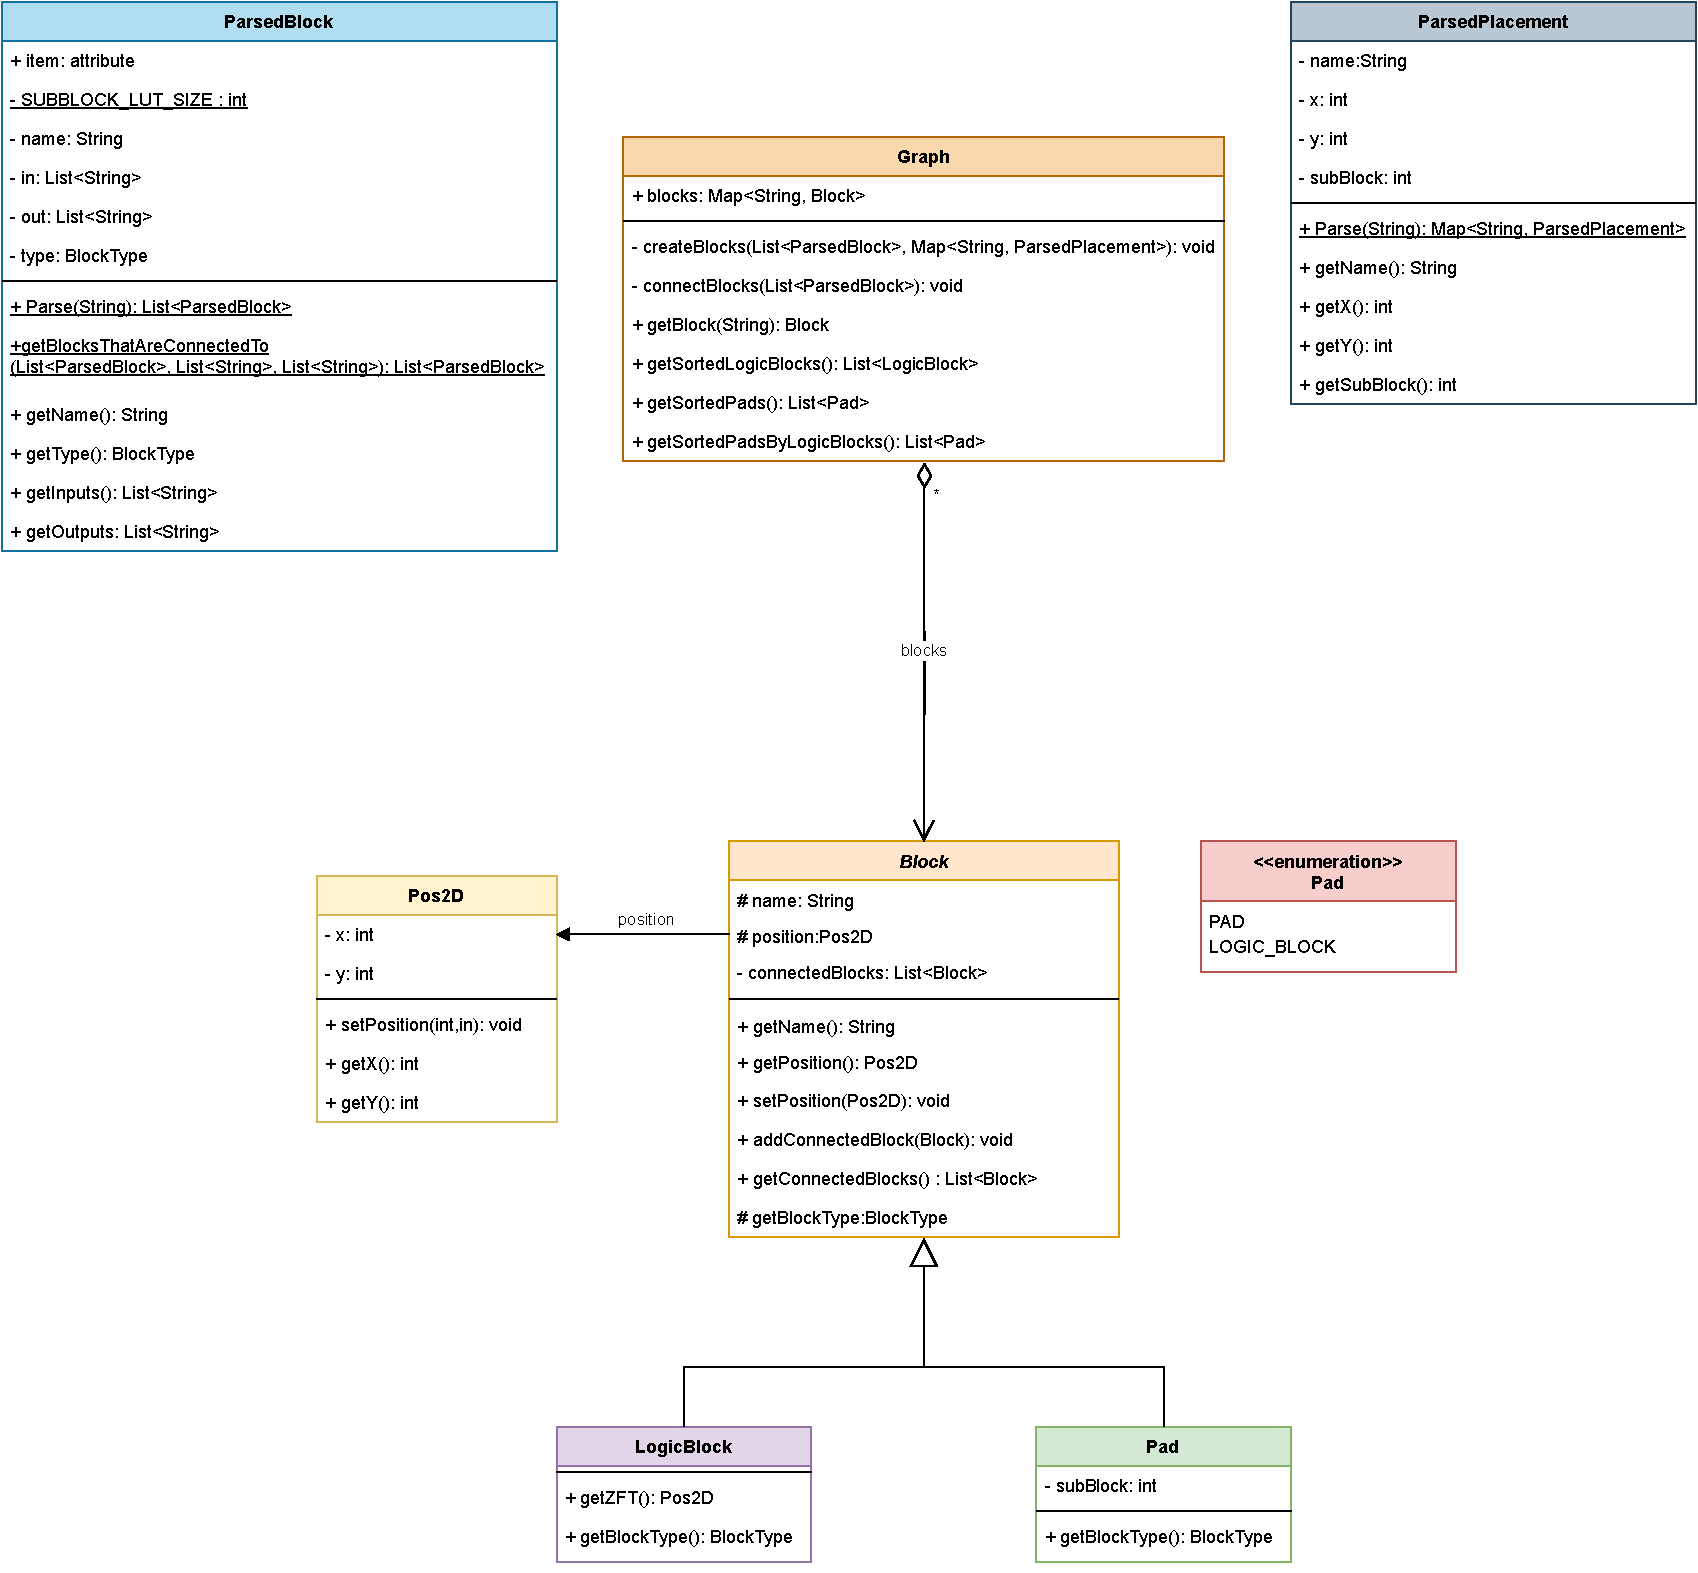
\includegraphics[width=\textwidth]{img/UML.pdf}
            \caption{UML Diagramm}
            \label{fig:uml}
        \end{figure}

    
        
    \section{Initialplatzierung}\label{sec:init}
        Dadurch, dass die Kräfteplatzierung ein iterativer Algorithmus ist,
        müssen die Blöcke gesetzt sein, um die jeweilige ZFT-Position zu berechnen.
        Ein möglicher Ansatz ist es, die Blöcke zufällig zu platzieren.
        Der Vorteil dieser Lösung ist, dass dieses Verfahren einfach umgesetzt werden kann.
        Der eindeutige Nachteil liegt in einer potenziellen schlechten Initialplatzierung,
        welche die Laufzeit und Effektivität der Kräfteplatzierung beeinflussen kann.
        In dieser Arbeit wurde von einer zufälligen Platzierung abgesehen und ein Ansatz gewählt,
        in dem die Logikblöcke nach Möglichkeit direkt auf ihre entsprechende ZFT-Position gesetzt werden.
        Die Problematik ist dabei, dass zur Berechnung der ZFT-Position mindestens zwei Blöcke,
        die mit dem zu platzierenden Block verbunden sind, bereits gesetzt sein müssen.
        Dies ist jedoch im Initialzustand nicht gegeben. Eine Lösung dieses Problems sind die Pads,
        die bereits bei der Konstruktion des Graphens an ihren entsprechenden Positionen fixiert werden.
        \\
        Der Ablauf der Initialplatzierung wird in Abbildung (\ref{fig:init-flowchart}) dargestellt.
        Zunächst wird eine Liste mit den zu platzierenden Logikblöcken absteigend nach ihrem
        Verbindungsgrad erstellt. Dies erhöht die Wahrscheinlichkeit, in den ersten
        Iterationsschritten Blöcke zu platzieren, die mit mehr als zwei fixierten Pads verbunden sind.
        Des Weiteren wird eine Zählervariable auf die Anzahl der zu platzierenden Blöcke gesetzt.
        Als Nächstes werden der Reihe nach Blöcke aus der Liste entnommen und zunächst geprüft,
        ob diese schon platziert wurden. Ist dies der Fall, wird der nächste Block aus der Liste entnommen.
        Wurde der Block jedoch noch nicht platziert, wird die ZFT-Position des Blockes ermittelt und geprüft,
        ob diese der Initialplatzierung (-1, -1) entspricht. In diesem Fall ist der Block mit zu wenig
        Blöcken verbunden, die bereits platziert sind und die ZFT-Postion kann zurzeit nicht ermittelt werden. 
        Ist dies nicht der Fall wird der Vorgang mit dem nächsten Block versucht. Kann jedoch eine valide
        ZFT-Position ermittelt werden, wird zunächst geprüft, ob diese bereits belegt ist.
        In solch einem Fall wird die nächste freie Position um die Zielposition gesucht und der
        Block auf diese gesetzt. Ist die Zielposition jedoch, kann der Block direkt gesetzt werden.
        In beiden Fällen wir der \textit{unset\_counter} dekrementiert und die Schleife versucht den nächsten Block
        zu platzieren.
        \\\\
        Ein Nachteil dieser Lösung ist, dass die berechnete ZFT-Position eines Blockes nicht zwangsläufig
        der korrekten ZFT-Position entspricht. Dies ist dadurch zu erklären, dass zum Zeitpunkt der
        Positionberechnung noch nicht alle verbundenen Blöcke platziert sind und somit das Ergebnis
        verfälscht wird.


        \begin{figure}[H]
            \centering
            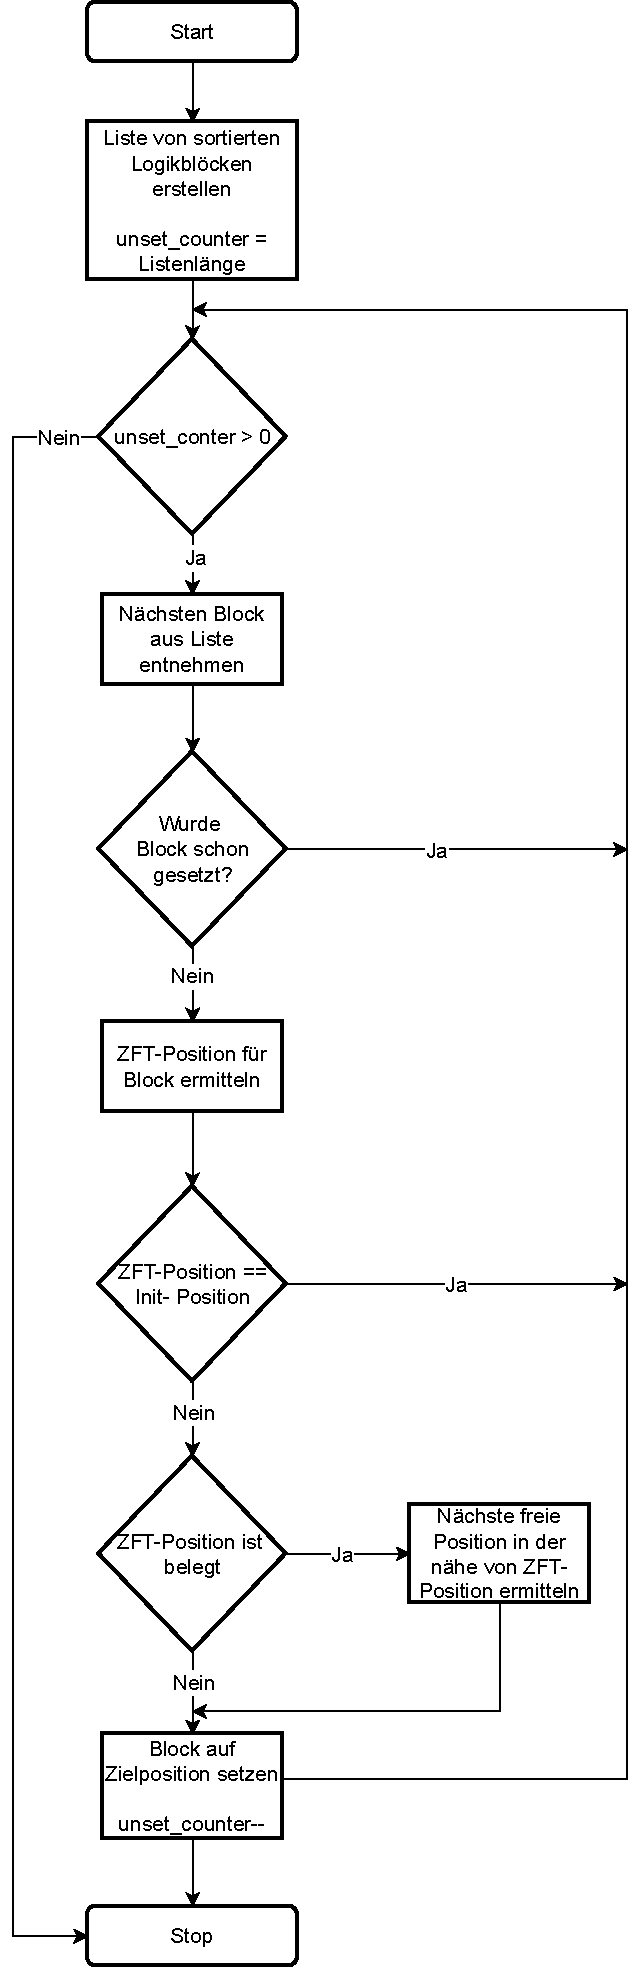
\includegraphics[scale=0.6]{img/init-flowchart.pdf}
            \caption{Initialplatzierung Ablaufplan}
            \label{fig:init-flowchart}
        \end{figure}

     

    \section{Ripple move}\label{sec:algo}
        Zunächst werden die Logikblöcke absteigend nach ihrem Verbindungsgrad sortiert.
        Das heißt, dass Blöcke mit mehr Verbindungen weiter vorne in der Liste stehen.
        Dies hat den Vorteil, dass diese Blöcke besser platziert werden können.
        Als Nächstes werden die Blöcke iterativ durchlaufen und für jeden Block die ZFT-Position ermittelt.
        \\
        Ist die Zielposition schon fixiert, das heißt, dass ein anderer Block in
        diesem Iterationsschritt auf die Zielposition gesetzt wurde, wird
        der \textit{rippleIteration} Zähler erhöht und verglichen,
        ob dieser größer bzw. gleich der \textit{maxRippleIteration} Variable ist.
        Ist dies der Fall, wird in der Nähe der Zielposition die nächste freie
        Zelle gesucht und der aktuelle Block auf diese Position gesetzt.
        Des Weiteren wird die maxIteration Zählervariable dekrementiert,
        alle Fixierungen werden gelöst und der Algorithmus beginnt eine neue Iteration. 
        \\
        In dem Fall, dass die \textit{maxRippleIterations} nicht überschritten wurde,
        wird die beste Position in der Nähe der Zielposition gesucht.
        Dabei werden alle anliegenden Positionen betrachtet und die Position ausgewählt,
        an dem der aktuelle Block der niedrigsten Kraft ausgesetzt ist.
        Die neue Zielposition wird daraufhin wieder auf die drei Hauptbedingungen geprüft.
        \\
        Ist die Zielposition nicht fixiert und der Block ist schon auf seiner Zielposition,
        wird die \textit{rippleIteration} Variable zurückgesetzt und die Zielposition fixiert.
        \\
        Ist die Zielposition jedoch belegt und nicht fixiert, wird der aktuelle Block
        auf die Zielposition gesetzt, die Position fixiert, der \textit{rippleIteration} Zähler zurückgesetzt
        und der verdrängte Block wird auf den aktuellen Block gesetzt.
        Als Nächstes startet der Algorithmus an der Stelle, an dem die ZFT-Position für den
        aktuellen Block (verdrängter Block) berechnet wird.\\
        Als letzte Bedingung kann die Zielposition unbelegt sein.
        Ist dies der Fall, wird der aktuelle Block auf die Zielposition gesetzt,
        die Position fixiert und der \textit{rippleIteration} Zähler zurück gesetzt.
        Ist der \textit{maxIterations} auf Null dekrementiert worden, wird der Algorithmus beendet.

        \begin{figure}[H]
            \centering
            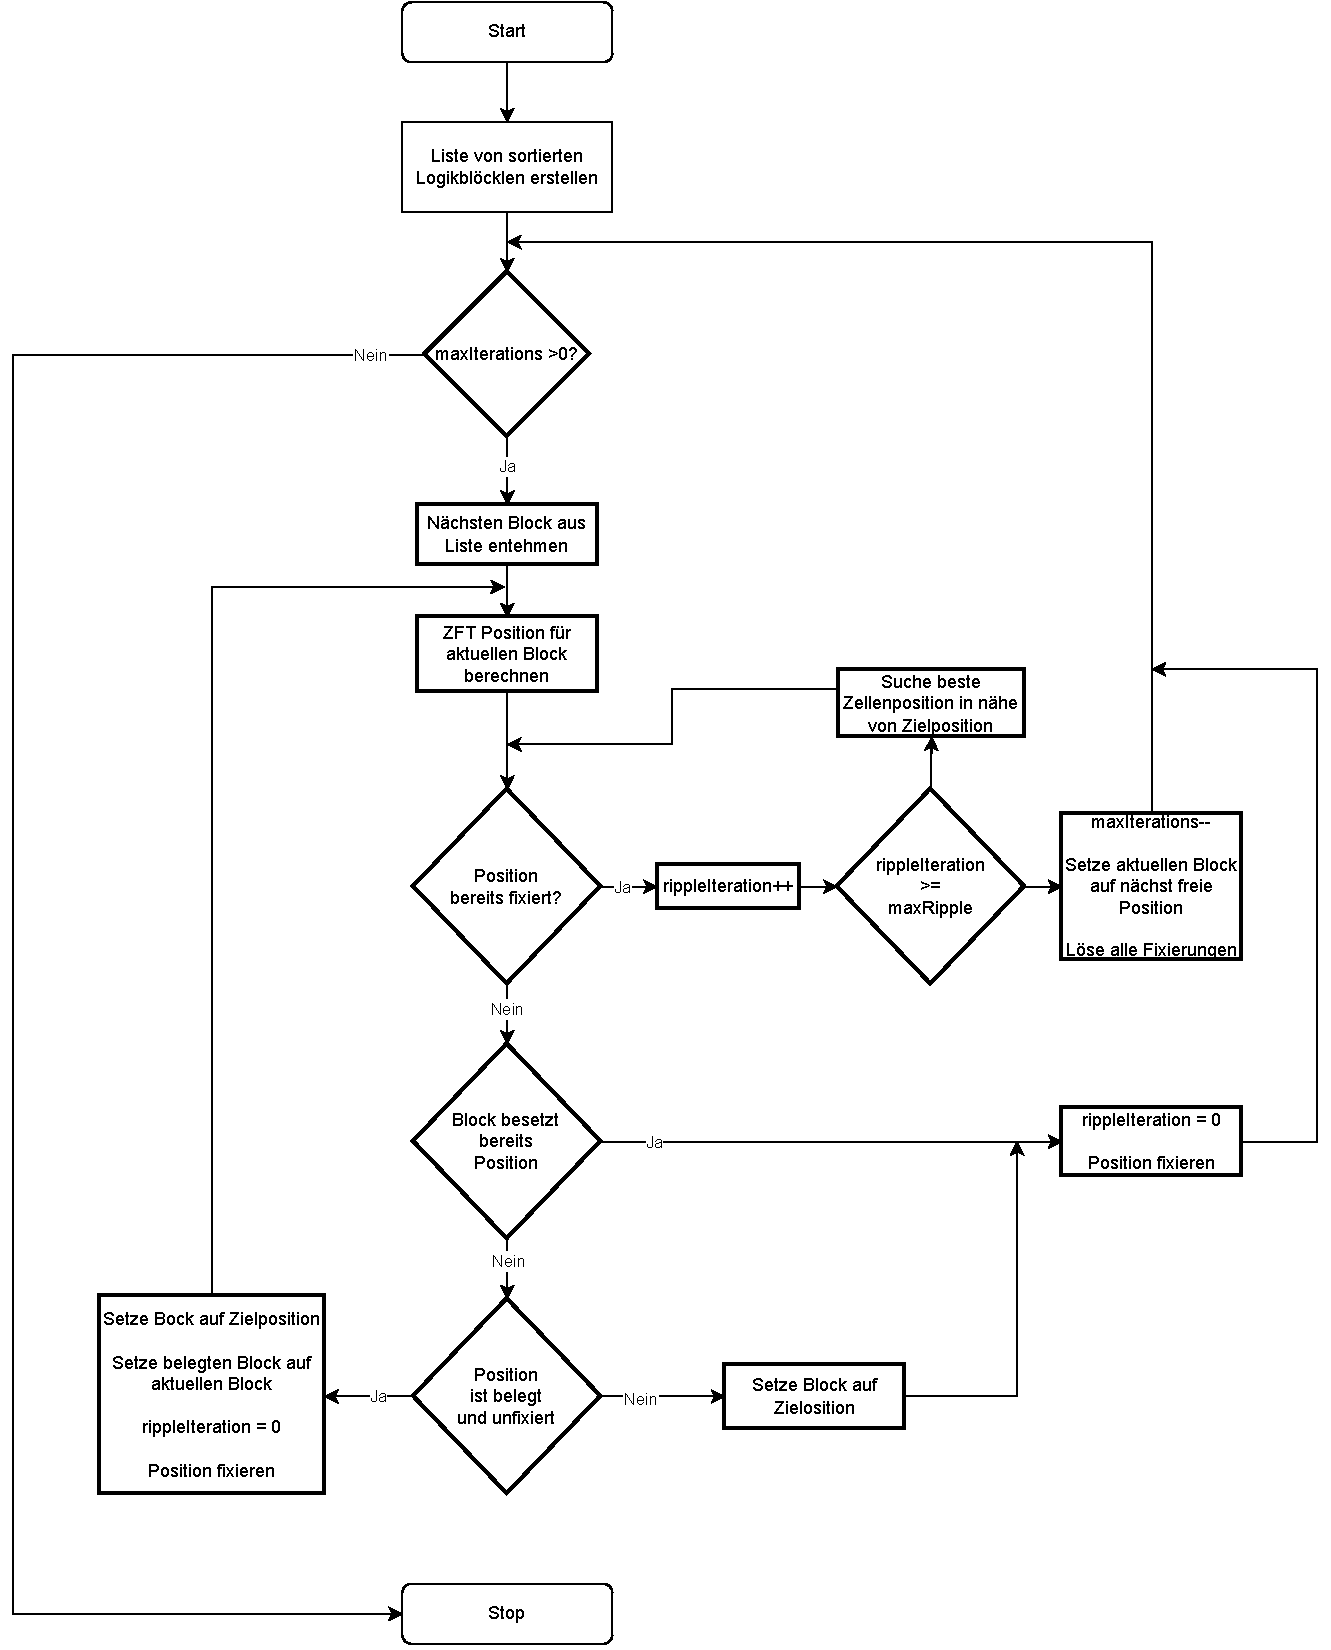
\includegraphics[width=\textwidth]{img/flowchart.pdf}
            \caption{Ripplemove Ablaufplan}
            \label{fig:algo-flowchart}
        \end{figure}
        Ein Nachteil von Algorithmen, die nach diesem Modell arbeiten, ist,
        dass sie dazu tendieren, alle Blöcke auf dieselbe Position zu setzen.
        Wenn eine Position jedoch schon belegt ist, muss eine andere und in diesem
        Fall auch schlechtere Position gesucht werden, sodass ein suboptimales
        Endergebnis zu erwarten ist. Des Weiteren ist zu erwähnen, dass in dieser
        Implementation die Gewichtungen der Verbindungen alle gleich sind.
        Das heißt, es gibt keine Blöcke bzw. Verbindungen, die priorisiert werden.
        Weiterhin werden in der aktuellen Implementation Blöcke an Zielpositionen
        verschoben, ohne dass die Kostendifferenz der Vertauschung berücksichtigt werden.
        Auch dies führt zu einem potenziell schlechteren Ergebnis.
        Darüber hinaus ist nicht zwangsläufig gegeben, dass ein Block an seiner
        ZFT-Position eine minimale Verdahtungslänge aufweisen.
        Das bedeutet, dass selbst wenn der Algorithmus jeden Block auf seine
        ZFT-Position platzieren kann, das Ergebnis nicht optimal sein muss.
        All diese Punkte müssen im Folgekapitel, insbesondere im Vergleich mit den
        Ergebnissen von VPR berücksichtigt werden.


